\documentclass{article}
\usepackage{amsmath, fullpage}
\usepackage[portuguese]{babel}
\usepackage{graphicx}
\usepackage{color}
\usepackage[normalem]{ulem}

\usepackage{listings}
\newcommand{\uvec}[1]{\boldsymbol{\hat{\textit{#1}}}}
\graphicspath{{image/}}
\newcommand{\stkout}[1]{\ifmmode\text{\sout{\ensuremath{#1}}}\else\sout{#1}\fi}

\begin{document}

\newcounter{boxlblcounter}  
\newcommand{\makeboxlabel}[1]{\fbox{#1.}\hfill}% \hfill fills the label box
\newenvironment{boxlabel}
  {\begin{list}
    {\arabic{boxlblcounter}}
    {\usecounter{boxlblcounter}
     \setlength{\labelwidth}{3em}
     \setlength{\labelsep}{0em}
     \setlength{\itemsep}{2pt}
     \setlength{\leftmargin}{1.5cm}
     \setlength{\rightmargin}{2cm}
     \setlength{\itemindent}{0em} 
     \let\makelabel=\makeboxlabel
    }
  }
{\end{list}}

\newenvironment{boxedd}
    {
     \begin{center}
    \begin{tabular}{|p{1\textwidth}|}
    \hline
    }
    { 
    \\\\\hline
    \end{tabular} 
    \end{center}
    }



\title{Sinais e Sistemas}
\author{Henrique de O. Bernardes}
%\date{\vspace{-5ex}}
\maketitle
\thispagestyle{empty}
\section{Aula 1a}
\textbf{Sinais} são quantidades ou grandezas que variam no tempo ou no espaço e carregam informações sobre o comportamento de fenômenos naturais ou artificiais. Ou seja, um \textbf{sinal} é a representação de como uma grandeza física (dependente) varia em relação a uma outra grandeza física (independente), transportando, assim, informação.

Um sinal pode representar, por exemplo:
\begin{enumerate}
  \item A variação de temperatura ao longo de um dia;
  \item A tensão elétrica em um circuito;
  \item A pressão sonora de uma música;
  \item A bolsa de valores ao longo do tempo.
\end{enumerate}

\textbf{Sistemas}, por sua vez, são estruturas ou processos que operam sobre sinais de entrada para produzir sinais de saída, seguindo um conjunto específico de regras ou comportamentos.
Um sistema pode ser tão simples quanto um amplificador que multiplica um sinal por uma constante ou tão complexo quanto um processador digital que realiza diversas operações em sinais de áudio ou vídeo.

\subsection{Sinal 1}
O primeiro sinal a ser analizado representa como o parâmetro dependente tensão \(y=f(t)\) varia em relação ao parâmetro independente tempo (\(t\), em segundos). Esta tensão representa 1 segundo da duração de um sinal de música.
\begin{boxedd}
\begin{lstlisting}
  >> [y, fs] = audioread("./Dados/music_sample3.wav");
  >> t=[0:length(y)-1]/fs;
  >> plot(t,y)
  >> grid on;
  >> axis([min(t), max(t)]);
\end{lstlisting}
\end{boxedd}
Primeiramente, fazemos a leitura do arquivo \textit{wav} por meio do comando \(audioread\), que nos retorna dois valores:
\begin{enumerate}
  \item \(y\), que representa os dados do audio, sendo armazenado como uma matriz onde as linhas correspondem aos frames de áudio e as colunas correspondem aos canais.
  \item \(f_s\), que representa o \textit{sampling rate}, ou taxa de amostragem, que representa o número de vezes por segundo que um valor é registrado.
\end{enumerate}
Definimos então a variável \(t\), definida como o tamanho do vetor \(y\) dividido por \(f_s\); ou seja, \(t\) nos diz em que instante de tempo cada ponto do áudio acontece, indo de 0 até o tempo total do áudio. 
Feito isso, plotamos o gráfico:
\begin{figure}[h!]
  \begin{center}
    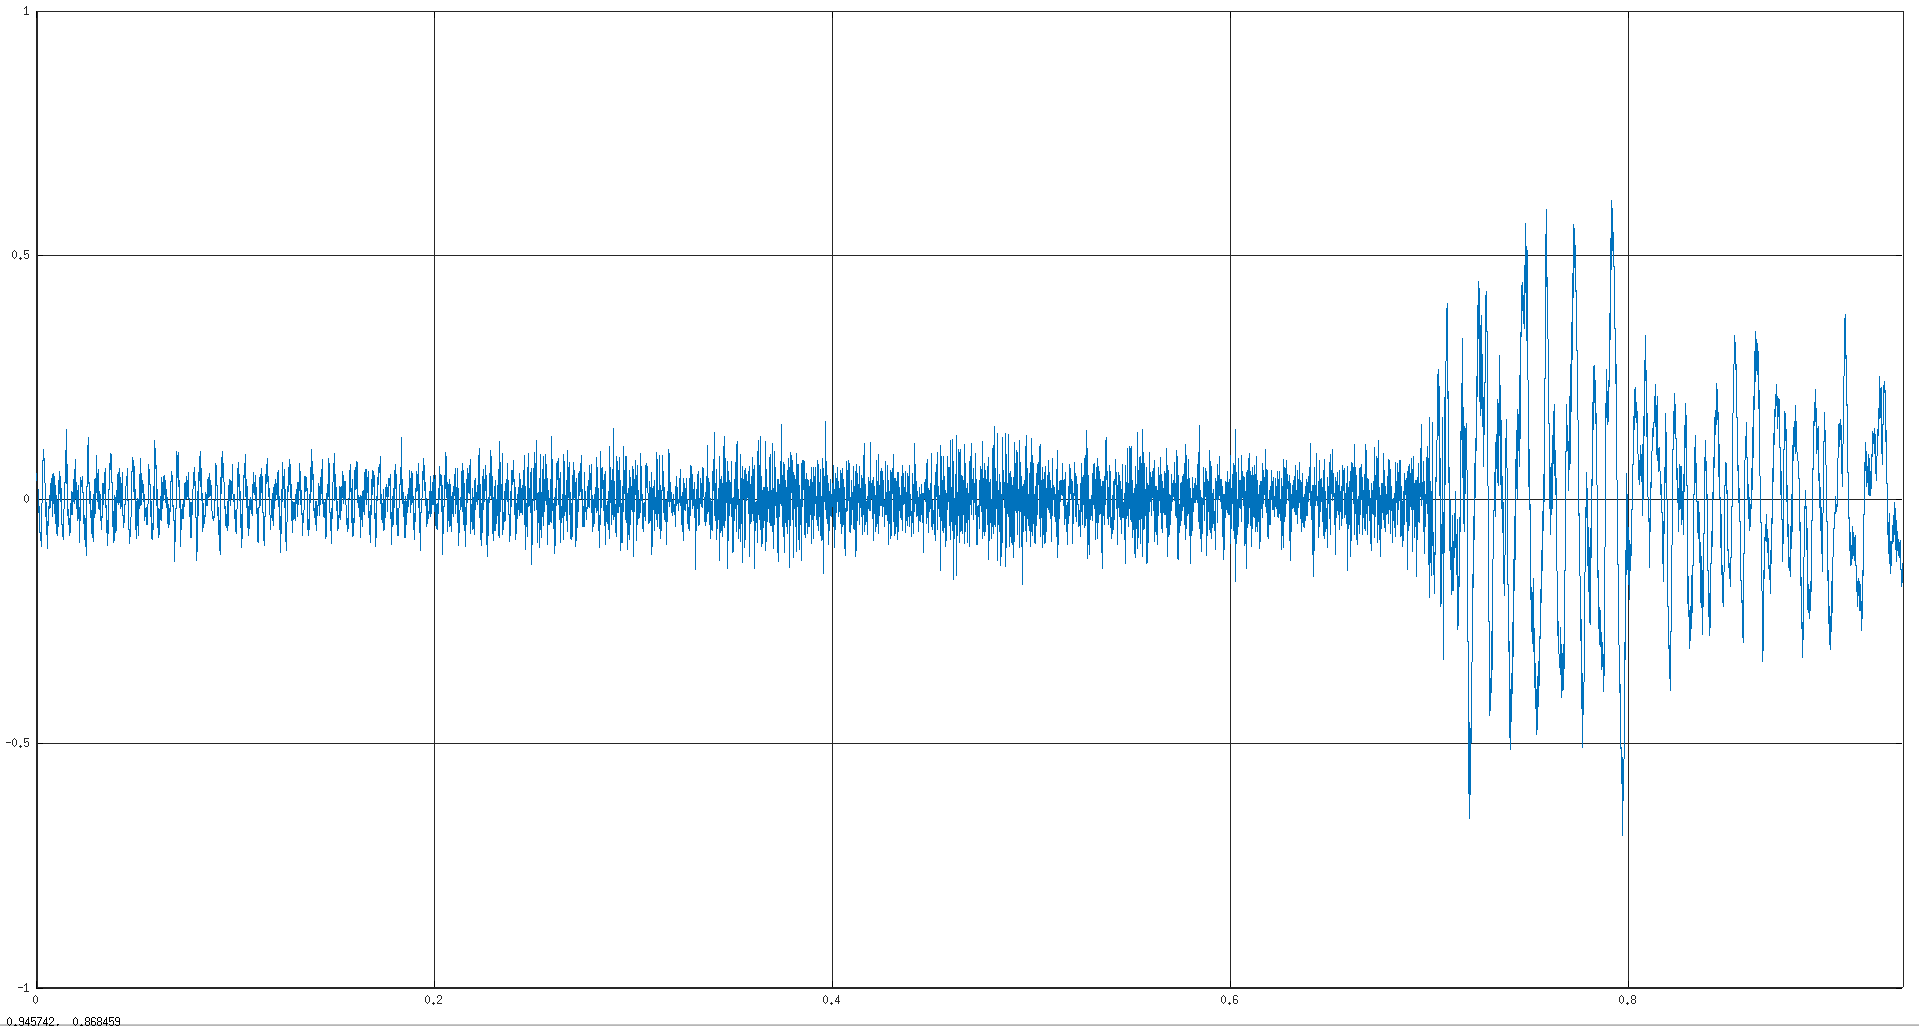
\includegraphics[width=0.7\textwidth]{figures/aula1a/sinal1.png}
  \end{center}
  \caption{Plot sinal 1}\label{fig:sinal1}
\end{figure}

Podemos, também, obter alguns dados extras:
\begin{boxedd}
\begin{lstlisting}
  >>T=1/fs
      T=1.25e-04
  >>n=length(y)
      n=7501
  >>l= n*T  
      l=0.9376
\end{lstlisting}
\end{boxedd}
Aqui, obtemos o período \(T\), que nada mais é do que o inverso da taxa de amostragem, e a duração total do sinal por meio da multiplicação do número total de amostras pelo período de cada amostra.
\newpage
\subsection{Sinal 2}
O segundo sinal diz como o parâmetro dependente altura da maré (em metros) varia em relação ao parâmetro independente tempo(em anos), nos mostrando como a maré do porto de Nova York se comporta ao longo de 150 anos.
\begin{boxedd}
\begin{lstlisting}
  >> [t, y] = textread("./Dados/MareNovaYork.txt", "%f %f", 1797);
  >> plot(t,y)
  >> grid on;
\end{lstlisting}
\end{boxedd}
Utilizando \textit{textread}, obtemos dois valores:
\begin{enumerate}
  \item \(t\), que representa o momento no tempo(ano e mês) em que a amostra foi capturada;
  \item \(y\), que representa a altura da maré naquele dado momento.
\end{enumerate}
Plotando esses valores, obtemos o seguinte gráfico:
\begin{figure}[h!]
  \begin{center}
    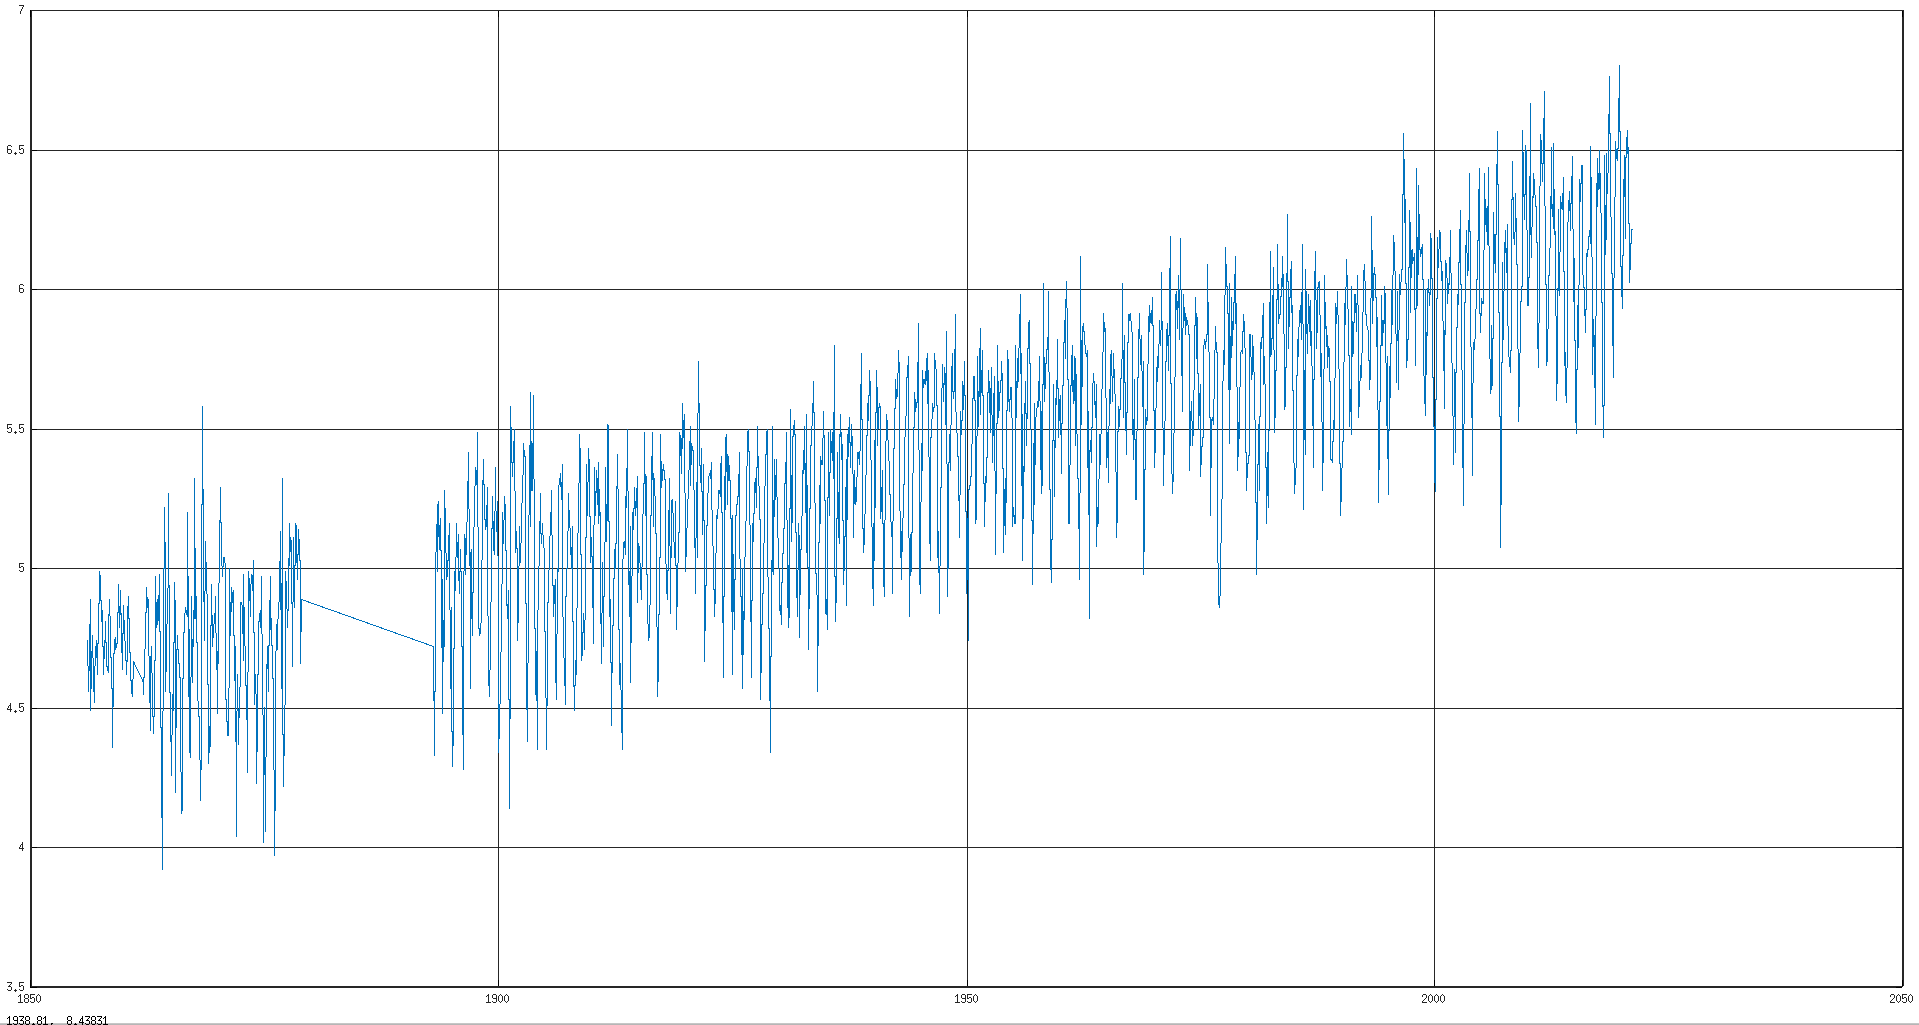
\includegraphics[width=0.7\textwidth]{figures/aula1a/sinal2.png}
  \end{center}
  \caption{Plot sinal 2}\label{fig:sinal2}
\end{figure}
Podemos obter, também, alguns dados extras como período, frequência, e duração total do sinal.
\begin{boxedd}
\begin{lstlisting}
  >> T=t(2)-t(1)
      T=0.083300
  >> fs=1/T
      fs=12.005
  >> n=length(y)
      n=1797
  >> l=n*T
      l=149.69
\end{lstlisting}
\end{boxedd}
\subsection
\iffalse
In this note, we will show how transformations can be used to obtain
a radically simple derivation of the equation of the line of best fit.
Our approach also gives a simple geometric interpretation of the Pearson
correlation coefficient.

Given a sequence of $n$ points in the plane $(X_1, Y_1), \ldots, (X_n, Y_n)$
we seek the linear equation $y = a + bx$ that approximates the points
as closely as possible, in the sense that the sum of the squared residuals
$E = \sum_{i=1}^n (Y_i - a - bX_i)^2$ is minimized.

We assume that not all of the points lie on a single horizontal or vertical
line. In that case, we can apply a \emph{transformation} to the points
so that $\sum x_i = \sum y_i = 0$ and $\sum x_i^2 = \sum y_i^2 = 1$.
The transformation is defined by
$$
x_i = \frac{X_i - \overline{X}}{\sqrt{\sum (X_i - \overline{X})^2}}\quad\text{and}\quad
y_i = \frac{Y_i - \overline{Y}}{\sqrt{\sum (Y_i - \overline{Y})^2}}.
$$

This transformation is linear, so it maps lines to lines.
If we transform a line fitted to the data,
the sum of squared residuals is multiplied by a positive constant factor.
Therefore, the transformation preserves the line of best fit.


Let $r = \sum x_i y_i$. Then
\begin{align*}
E &= \sum (y_i - a - bx_i)^2 \\
&= \sum (y_i^2 + a^2 + b^2 x_i^2 - 2ay_i - 2bx_iy_i + 2abx_i) \\
&= \sum y_i^2 + \sum a^2 + \sum b^2 x_i^2 
 - \sum 2ay_i - \sum 2bx_iy_i + \sum 2abx_i \\
&= 1 + na^2 + b^2 - 2br \\
&= (1-r^2) + na^2 + (b - r)^2\ .
\end{align*}

The sum is minimized when $a = 0$ and $b = r$, so the line of best fit is
$y = rx$. What a simple equation!
Unfortunately, the equation is a bit messier when expressed in terms of the
original variables.

\begin{align*}
\frac{y - \overline{Y}}{\sqrt{\sum (Y_i - \overline{Y})^2}}
&= \left(
     \frac{\sum (X_i - \overline{X}) (Y_i - \overline{Y})}
          {\sqrt{\sum (X_i - \overline{X})^2 \sum (Y_i - \overline{Y})^2}}
   \right)
   \left(
     \frac{x - \overline{X}}
          {\sqrt{\sum (X_i - \overline{X})^2}}
   \right)\\
y - \overline{Y} &=
\left(
     \frac{\sum (X_i - \overline{X}) (Y_i - \overline{Y})}
          {\sum (X_i - \overline{X})^2}
   \right)
   (x - \overline{X})\ .
\end{align*}

Note that $r$ is the Pearson correlation coefficient of the sample.
This shows that the correlation coefficient can be interpreted geometrically
as the slope of the line of best fit when the $x$ and $y$ values are standardized.
\fi


\end{document}
